% !TeX spellcheck = en_US
\section{Problem 9}

In figure~\ref{fig:prob9_given_contour_plot}, we are given a contour plot and we are asked to draw one gradient step for the three following algorithms:
\begin{itemize}
	\item Gradient Descent,
	\item Natural Gradient (\textit{Newton's method}) and
	\item Adagrad or RMSprop.
\end{itemize}

\begin{figure}[htpb]
	\centering
	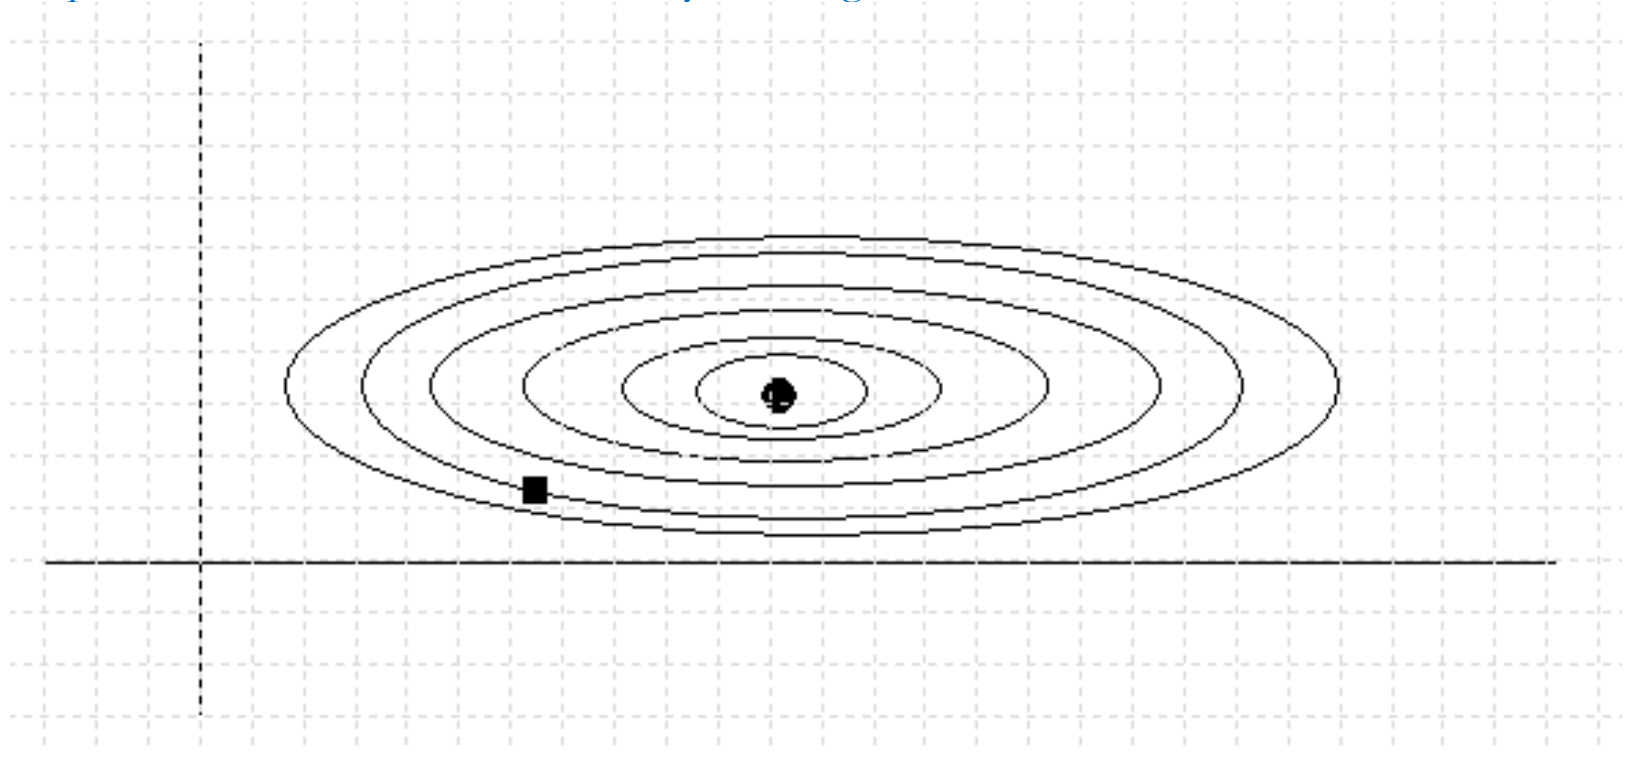
\includegraphics[width=0.7\textwidth]{../Problem 9/contour_plot.png}
	\caption{Given contour plot.}
	\label{fig:prob9_given_contour_plot}
\end{figure}

\subsection{Gradient Descent}

Gradient Descent calculates the next step as follows. First, the gradient is calculated using a \textit{mathematical expression}. Then, it progresses through the contour plot in the opposite direction of gradient.

This is done repeatedly, until a local minimum is found and converges there.\\

In this problem, we don't have any mathematical expression in order to calculate the gradient, so we will approximate it \underline{visually} from the contour plot.

Looking at the starting point in figure~\ref{fig:prob9_given_contour_plot} (\textit{the rectangle}), 
the gradient at this point is perpendicular to the contour line and points in the direction of the steepest increase in function value, which is the area where contour lines are closer to each other.\\
Following the algorithm, gradient descent moves in the \textit{opposite direction of the gradient}, which is the direction of the steepest decrease in function value.

Gradient and direction of movement are shown in figure~\ref{fig:prob9_contour_gd}.

\begin{figure}[htpb]
	\centering
	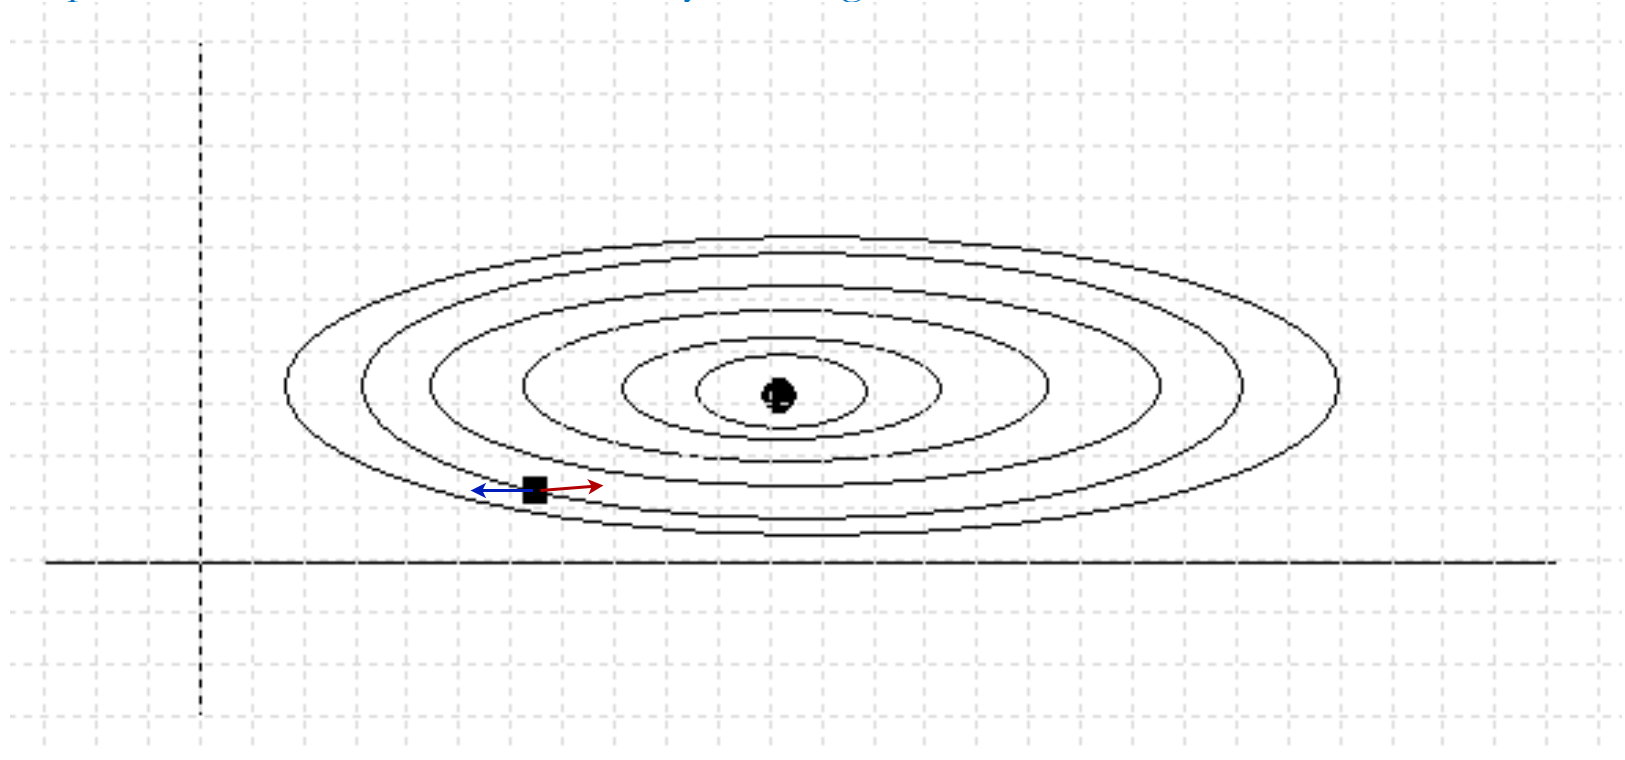
\includegraphics[width=0.7\textwidth]{../Problem 9/contour_gd.png}
	\caption{First step of gradient descent. Blue arrow represents the \textbf{gradient} on the first step and red arrow represents the \textbf{step} of the algorithm.}
	\label{fig:prob9_contour_gd}
\end{figure}


\subsection{Newton's Method}

Newton's method is an optimization method that takes into account the information about the curvature of the function, which allows it to make a more informed step towards the minimum.

The natural gradient is adjusted by taking into consideration the inverse of the Hessian, a matrix of all second-order partial derivatives of the function. 
The steps are more direct and perhaps longer, pointing straight toward the minimum because these methods are designed to take the most direct route in the parameter space considering the curvature.\\

Again, we don't have any expression for the function in order to calculate directly the gradient (\textit{and every other factor}), thus we are going to approximate it visually.

The first step for Newton's method is to calculate the gradient, which can be obtained from \textbf{Gradient Descend} calculations.

Next step is to factor in the curvature of the space. Because of the high curvature in this area, step's size is going to be smaller than Gradient Descent's one.\\

So, the approximated step of Netwon's Method is shown in figure~\ref{fig:prob9_contour_newtons}.

\begin{figure}[htpb]
	\centering
	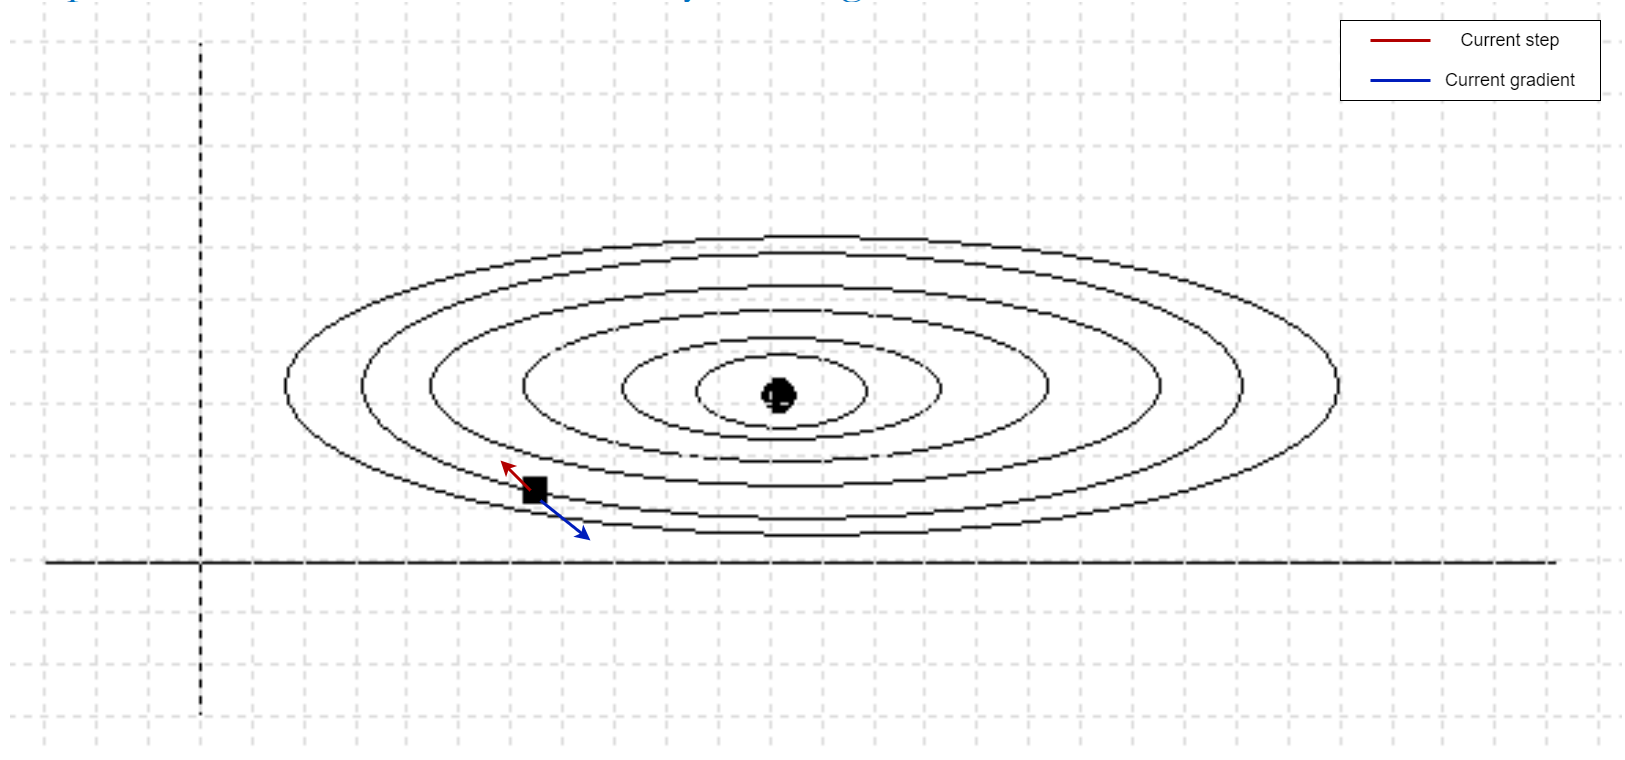
\includegraphics[width=0.7\textwidth]{../Problem 9/contour_newtons.png}
		\caption{First step of Newton's Method. Blue arrow represents the \textbf{gradient} on the first step and red arrow represents the \textbf{step} of the algorithm.}
	\label{fig:prob9_contour_newtons}
\end{figure}

\subsection{Adagrad / RMSprop}

Adagrad is an optimization algorithm designed to adapt the learning rate to the parameters, performing smaller updates for parameters associated with frequently occurring features and larger updates for parameters associated with infrequent features. 

It offers an adaptive learning rate where each parameter has its own learning rate, improving performance on problems with sparse gradients. \\

RMSprop is also an adaptive learning rate method that solves a weakness of Adagrad. RMSProp addresses Adagrad's radically diminishing learning rates by using a moving average of squared gradients. This ensures that the learning rate does not decrease too rapidly and is adapted for each weight.\\

For both Adagrad and RMSProp, the initial direction of movement is opposite to the gradient at the current point. After this point, the two algorithms differentiate. Adagrad decreases the learning rate for each parameter based on the sum of the squares of past gradients for that parameter but this can lead to very small step sizes.\\

RMSprop modifies Adagrad's approach by using a moving average of the squared gradients instead, which prevents the learning rate from diminishing too rapidly. This means that, compared to Adagrad, RMSProp can maintain a larger step size in areas where Adagrad's steps might become excessively small.

If we assume that they have run for a while to accumulate gradient
information, then the step of Adagrad will be a lot smaller than that of RMSprop.

Thus, the approximated steps for Adagrad and RMSprop are shown in figure~\ref{fig:prob9_contour_adagrad_rmsprop}.

\begin{figure}[H]
	\centering
	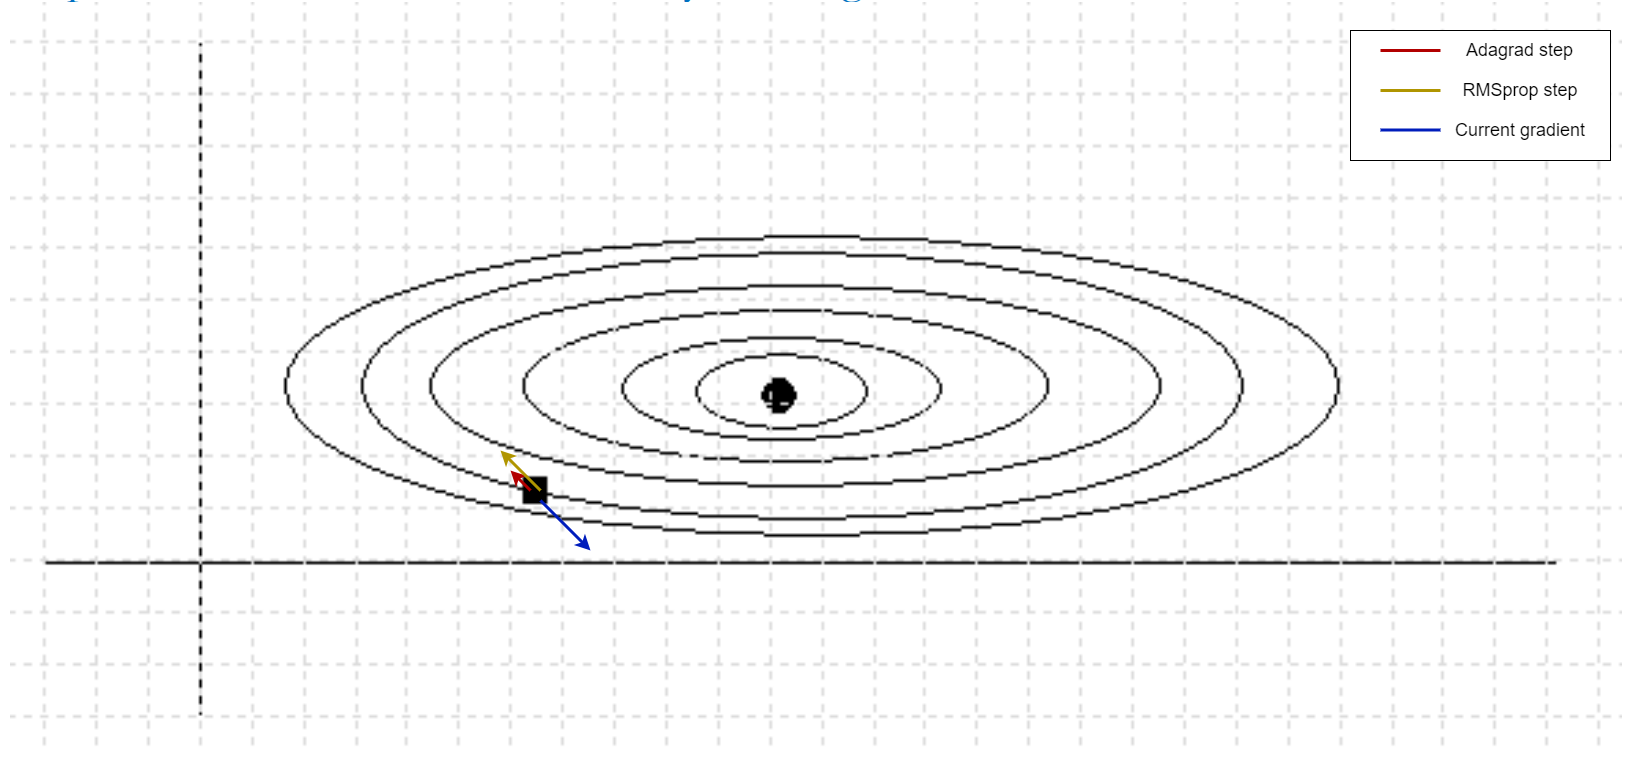
\includegraphics[width=.7\textwidth]{../Problem 9/contour_adagrad_rmsprop.png}
	\caption{First step of Adagrad and RMSProp (*). Blue arrow represents the \textbf{gradient} on the first step and red arrow represents the \textbf{step} of the algorithm.\\
	\textit{\small(*): Here, it is assumed that the algorithms have learned about the gradients a bit.\\ Also, both steps are parallel.}
	}
	\label{fig:prob9_contour_adagrad_rmsprop}
\end{figure}
\vspace{3mm}